\documentclass[a4paper,12pt]{article}
\usepackage[utf8]{inputenc}
\usepackage[ngerman]{babel}
\usepackage[top=1in, bottom=1.25in, left=1.25in, right=1.25in]{geometry}
\usepackage{minted}
\usepackage{blindtext}
\usepackage{fancyhdr}
\usepackage{titling}
\usepackage{amssymb}
\usepackage{mathtools}
\usepackage{enumitem}
\usepackage{hyperref}
\usepackage{csquotes}
\MakeOuterQuote{"}

\hypersetup{colorlinks=true,linkcolor=blue,urlcolor=blue}

\renewcommand{\footrulewidth}{0.4pt}

\setlength\headheight{15pt}
\setlength{\parskip}{1em}

\title{GNS Aufgabe 2}
\author{Eli Kogan-Wang}
\date{\today}

\pagestyle{fancy}
\fancyhf{}
\lhead{\thetitle}
\rhead{\thedate}
\lfoot{\theauthor}
\rfoot{Page \thepage}


\begin{document}
% \maketitle
% \thispagestyle{fancy}

\section{Inhaltliche Organisation}
\textbf{Beurteilen Sie die Startseite der Universität Paderborn
  (https://www.uni-paderborn.de/) nach den folgenden in der Vorlesung behandelten
  Organisationsprinzipien der Informationsarchitektur:}
\begin{enumerate}[label=\alph*)]
  \item \textbf{Sind die häufig verwendeten Elemente auf der Seite sichtbar und an
          offensichtlichen Stellen? Erläutern Sie in 3-4 Sätzen, warum Sie mit Ja oder
          Nein geantwortet haben.}

        Die Startseite der Universität Paderborn fungiert als Index über Informationen über die Universität.
        Auf meinen Bildschirm sind als Interaktionselemente sichtbar:

        Schnellzugriff, Kontakt, DE/EN, Suche \\
        Studium, Lehre, Forschung, Universität, Fakultäten (als Navbar) \\
        Studieninteressierte, (etc...)\\
        Nachrichten, Veranstaltungen

        Ich sage \textbf{Nein}. Denn die häufig verwendeten Elemente sind die Links \textit{hinter} den
        sofort sichtbaren Interaktionselementen, und somit hinter einem such/browse Schritt versteckt.
        Die Interaktionselemente, die sichtbar sind, sind ein Mittel zum Zweck, um die häufig
        verwendeten Elemente zu kategorisieren.

  \item \textbf{Öffnen Sie die Website auf Ihrem mobilen Gerät. Wie sieht die Webseite auf
          einem mobilen Gerät aus? Unterscheidet sich das Erlebnis von dem auf dem
          Desktop? Warum?}

        Die Website sieht ähnlich strukturiert aus. Die Punkte Studium, [...], Alumni sind
        hinter einem Hamburger Menü versteckt. Häufig verwendete Elemente sind also
        hinter einem weiterem Such/Browse Schritt versteckt.

        Die Entscheidung die Elemente in einem Hamburger Menü zu verstecken ist
        in Bezug der Bildschirmgröße und des Formats des Bildschirms sinnvoll.
        Dadurch wird Platz gespart, sodass Nachrichten und Veranstaltungen
        auf dem Bildschirm immer noch sichtbar sind.

  \item \textbf{Wie würden Sie den Inhalt der Webseite umstrukturieren? Sie können für
          diese Frage auch Skizzen auf einem Papier oder einem digitalen Whiteboard
          anfertigen und einen Screenshot anhängen.}

        \begin{figure}
          \centering
          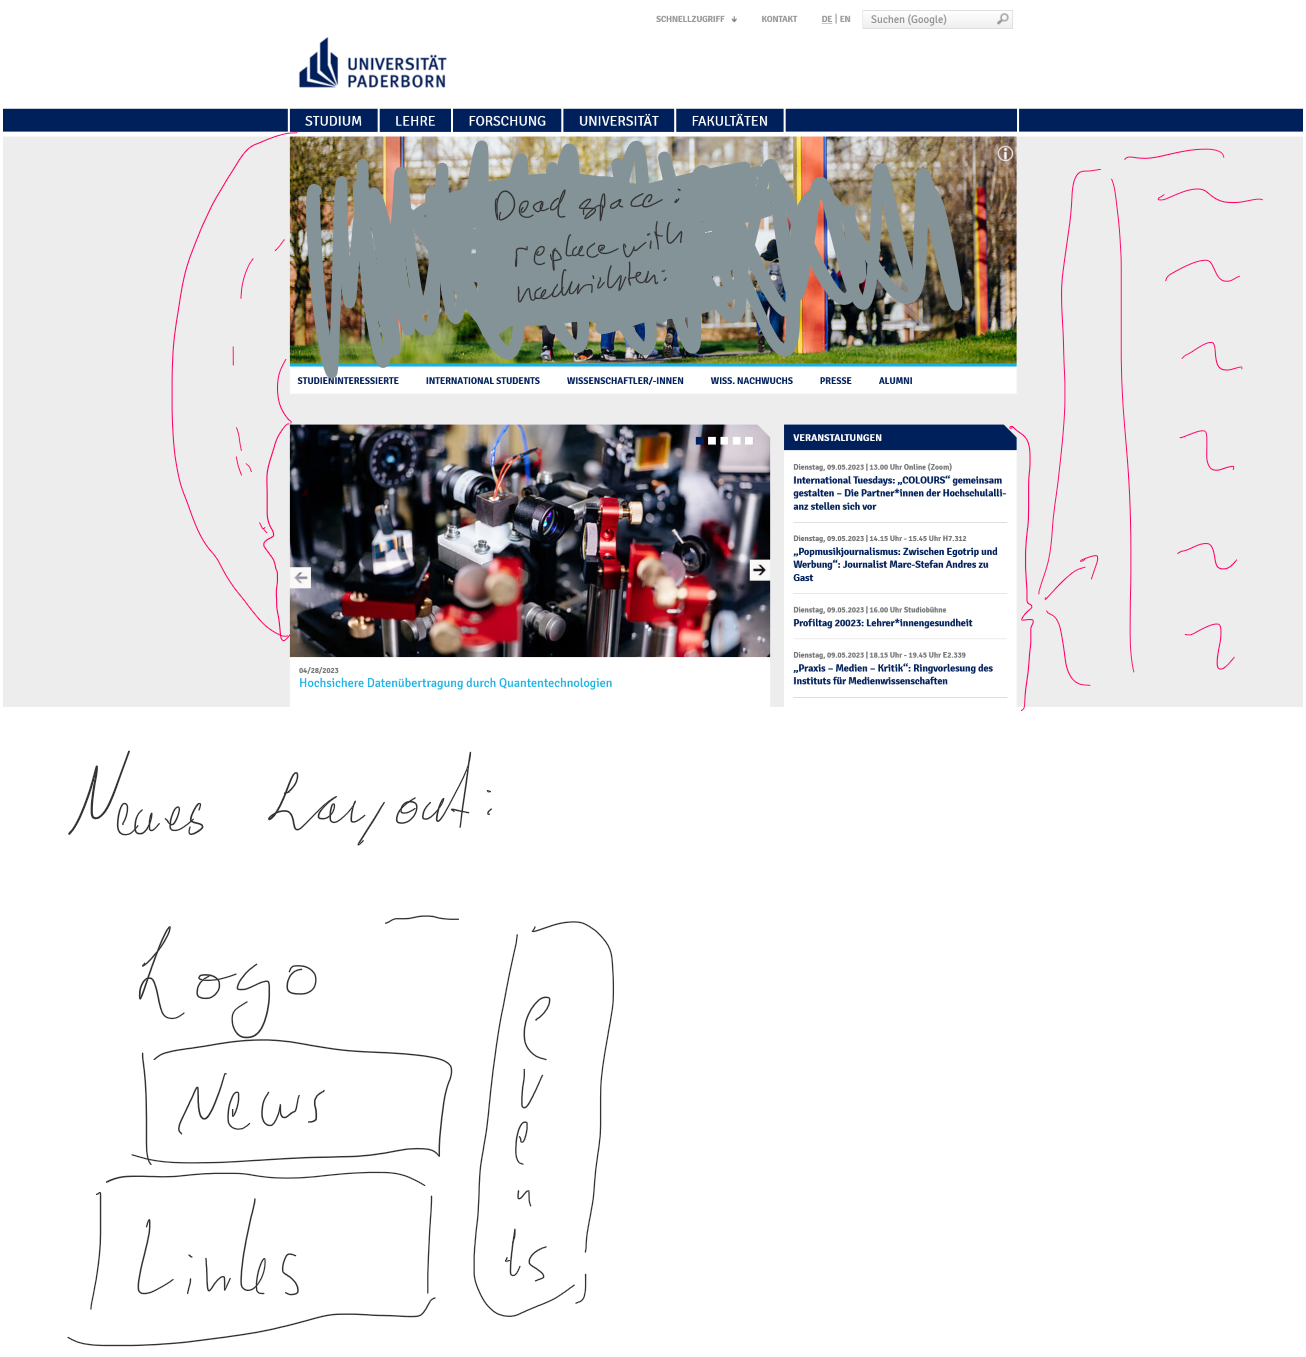
\includegraphics[width=0.8\textwidth]{./2023-05-08-4P5owdQYFDNH4AAAAASUVORK5CYII.png}
          \caption{Skizze der Startseite der Universität Paderborn}
        \end{figure}

        Mich stört der White Space auf der Startseite. Ich würde den Platz des
        White-Space Nutzen, um die Navbar auszuweiten, sodass die häufig
        verwendeten Elemente sichtbar sind.
\end{enumerate}


\section{Navigation}
\textbf{Beurteilen Sie die Navigation von Der Spiegel (https://www.spiegel.de/)
  anhand der in der Vorlesung behandelten Gestaltungsprinzipien für die
  Navigation. Schreiben Sie eine Kritik der Navigation, betrachten Sie
  sowohl die globale Navigation als auch die Navigation im Burger-Menü und
  erklären Sie, ob diese den folgenden Prinzipien folgen oder dagegen
  verstoßen (erklären Sie mindestens 2 Prinzipien):}

% i. Trennen Sie das Navigationsdesign vom visuellen Design
% ii. Gruppieren Sie ähnliche Elemente zusammen
% iii. Reduzieren Sie die kognitive Belastung
% iv. Halten Sie die Wege kurz / Halten Sie die Anzahl der Taps und Klicks
% klein
% v. Minimieren Sie die Anzahl der Hierarchien
% vi. Häufig aufgerufene Elemente können direkt in der globalen Navigation
% enthalten sein
% vii. Gemeinsame Aufgaben sollten auf einem einzigen Bildschirm erledigt
% werden können

Auf der Startseite besteht die sofort Sichtbare Navigation aus einer
Navbar, die die Punkte Menü, Schlagzeilen, Spiegel+, Magazine, Krieg in der Ukraine, [...] enthält.
Man bemerkt, dass die Punkte in der Navbar nicht alle derselben Kategorie von
Dingen angehören. Das kommt daher, dass \textbf{häufig verwendete Elemente direkt
  in der globalen Navigation eingebunden wurden}.

Auch ist ein Burger-Icon neben dem Punkt Menü sichtbar. Beim öffnen des
Burger-Menüs werden die Punkte der Navbar in einer vertikalen Liste angezeigt.
Dies verdoppelt die Anzahl der möglichen Interaktionen, um zu einem Punkt
zu gelangen. Damit wird die \textbf{kognitive Belastung erhöht}.

\section{Guter Inhalt und gute Navigation}
\textbf{Fügen Sie einen Link zu einer Website hinzu, die
  Ihrer Meinung nach eine gute Navigation und Inhaltsorganisation aufweist, und
  erklären Sie, warum. Sie können keine Social-Media-Plattformen, visuelle Seiten wie
  flickr oder printerest oder Seiten wie github verwenden. Die von Ihnen gewählte
  Webseite sollte über genügend Inhalt und eine klare Navigation verfügen (z. B.
  Nachrichtenseiten, Wikipedia, Landing Pages von Universitäten, staatliche Websites
  wie https://www.paderborn.de/).}

\url{https://ncatlab.org/nlab/show/HomePage} ist ein Wiki für Mathematik, besonders
Kategorientheorie. Die Landing-Page ist selbst eine Wiki-Seite, sodass diese
über den Wiki-Prozess aktuell gehalten wird. Die Startseite fungiert als Readme über
das Wiki und verfügt über Links in das Wiki, sodass eine Navigation in den Wiki-Graphen
zu den gewünschten Informationen möglich ist. Auch ist eine Suche vorhanden, sodass
ein Nutzer nach gewünschten Informationen suchen kann.

Das Wiki-Link-Graph-Navigationsformat ist eines der uns in der Vorlesung nicht
eingeführten Formate. Eine besonderheit dieses Formats ist, ist dass der Navigationsgraph
auch tiefergehende Informationen enthält.

\section{Visuelle Hierarchie}
\textbf{Wählen Sie eine Website oder App, die Sie häufig nutzen, und
  analysieren Sie deren visuelle Hierarchie. Welche Teile der ausgewählten App oder
  Website stechen am meisten hervor? Gibt es irgendwelche Verbesserungen oder
  Änderungen, die Sie vornehmen würden, um die visuelle Hierarchie effektiver zu
  gestalten? Wenn Sie keine Änderungen vornehmen würden, erklären Sie, warum die
  visuelle Hierarchie derzeit gut funktioniert.}

Ich verwende oft \url{https://mathoverflow.net/}. Die Seite ist ein Forum für
Mathematik-Fragen. Die Seite Navigiert sich im Hub-and-Spoke Format.

Es gibt die Startseite, Suchseite, und andere Seiten, die eine Liste von Fragen
enthalten. Diese Seiten fungieren als Hub-Seiten und Zeigen zu den Frage-Seiten.

Die Frage-Seiten präsentieren die Frage und die Antworten und sind damit die Inhalte, die
die Nutzer sehen wollen. Die Frage-Seiten sind die Spoke-Seiten. Bei Mathoverflow
ist das Format aber nicht so genau eingehalten, sodass die Frage-Seiten zu anderen
Frage-Seiten verlinken.

\section{Atomares Design}

\textbf{Erklären Sie, was Sie über atomares Design verstanden haben
  und warum es nützlich ist.}

Atomares Design ist ein Design-Prinzip, dass die Komponenten einer Website
in Atome, Moleküle, Organismen, Templates und Seiten einteilt.

In der Realität sind Atome die von der Plattform bereitgestellten UI-Elemente,
aus denen größere Komponenten zusammengesetzt werden. Die Abstraktionsstufen Moleküle
und Organismen sind subjektiv und können von Projekt zu Projekt variieren. Templates
sind die Komponenten, die über Seiten hinweg nützliche Funktionen bereitstellen. Seiten
sind die konkreten Darstellungs-kompositionen, die der Nutzer sieht.

So kann man beispielsweise in der Web-Plattform die Atome als HTML-Elemente sehen,
die Schichten Atome bis hin zu Seiten als Komponenten
(z.B. React oder Vue oder Angular oder Web- oder Svelte Components).

Die hierarchische Einteilung der Komponenten in Atome, Moleküle, Organismen, Templates
dient dabei der Aufgabentrennung beim Design und der Entwicklung.



\end{document}
